\section{Protocols}

\secttoc

The following abbreviations are used so the labels fit:

\begin{description}
  \item[OPeer] An Ordinary Peer
  \item[SPeer] A Super Peer
  \item[HCache] The Host Cache
  \item[Req] Request
  \item[Resp] Response
\end{description}

\subsection{Joining the network}

This involves contacting the Host Cache for the IDs of Super Peers, and
requesting a connection.  The connection can either be accepted or denied. If
the connection is accepted, the peer sends their list of shared files to the
connected Super Peer.

\noindent\makebox[\textwidth]{
  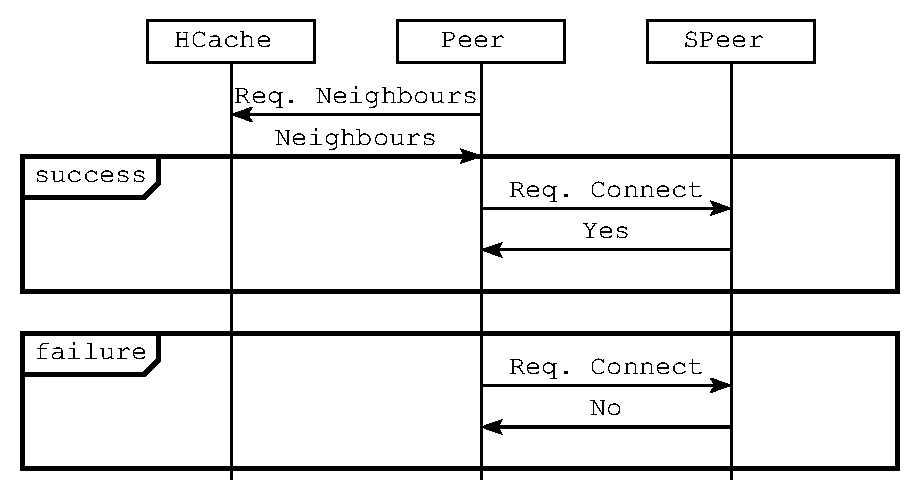
\includegraphics[max width=\textwidth]{protocol_connect.eps}
}

\subsection{Searching for Files}

In the following example, there are only two Super Peers in the network.  The
search request is forwarded throughout the network, and if at some point a Super
Peer is able to locate it, the location is passed back through the network to
the original requester.

\noindent\makebox[\textwidth]{
  \includegraphics[max width=\textwidth]{protocol_file_search.eps}
}

\subsection{Acquiring Files}

Once a file location has been determined, acquiring it is straightforward direct
communication between two peers.

\noindent\makebox[\textwidth]{
  \includegraphics[max width=\textwidth]{protocol_acquire_file.eps}
}

\subsection{Reporting Stats}

In order to gain insight into the state of the network, peers periodically (and
in response to certain conditions) send statistical information to a Runner
agent, which is also responsible for starting up all the peers in the
simulation.

\noindent\makebox[\textwidth]{
  \includegraphics[max width=\textwidth]{protocol_send_stats.eps}
}
